\documentclass[conference]{IEEEtran}
\IEEEoverridecommandlockouts
% The preceding line is only needed to identify funding in the first footnote. If that is unneeded, please comment it out.
\usepackage{cite}
\usepackage{amsmath,amssymb,amsfonts}
\usepackage{algorithmic}
\usepackage{graphicx}
\usepackage{textcomp}
\usepackage{hyperref}
\usepackage{xcolor}
\usepackage{float}

\usepackage{tabularx,booktabs}
\newcolumntype{C}{>{\centering\arraybackslash}X}
\setlength{\extrarowheight}{1pt} % for a bit more open "look"
\usepackage{graphicx}

\def\BibTeX{{\rm B\kern-.05em{\sc i\kern-.025em b}\kern-.08em
    T\kern-.1667em\lower.7ex\hbox{E}\kern-.125emX}}
\begin{document}

\title{Simple Reactive Robot\\
}

\author{

    \IEEEauthorblockN{Carlos Veríssimo}
    \IEEEauthorblockA{\textit{Department of Informatics Engineering} \\
        \textit{FEUP}\\
        Porto, Portugal \\
        up201907716@up.pt }
    \and

    \IEEEauthorblockN{Miguel Amorim}
    \IEEEauthorblockA{\textit{Department of Informatics Engineering } \\
        \textit{FEUP}\\
        Porto, Portugal \\
        up201907756@up.pt }
    \and

    \IEEEauthorblockN{Rafael Camelo}
    \IEEEauthorblockA{\textit{Department of Informatics Engineering } \\
        \textit{FEUP}\\
        Porto, Portugal \\
        up201907729@up.pt }
}


\maketitle

\begin{abstract}

    In an era defined by dynamic and ever-evolving technological landscapes, the development of a REACTIVE (Real-time, Environment-Adaptive, and Contextually-Intelligent) robot under the aegis of the Robot Operating System (ROS) represents a pivotal step forward in the realm of robotics. This ambitious project aspires to create a robotic entity with unparalleled adaptability, reactivity, and intelligence in response to its environment.  The simulation is performed in ROS, which runs the Python code and integrates it with the Gazebo simulation
    environment. The reactive robot is generated in a random start
    position. It can successfully follow the wall, avoid hitting, and stop
    in the desired end position.

\end{abstract}

\begin{IEEEkeywords}
    Robotics, Intelligent, ROS, Gazebo, Simulation, Sensor, Actuator, Navigation, Environment
\end{IEEEkeywords}

\section{Introduction}
As technology continues to advance, autonomous mobile robots are increasingly finding applications across various sectors, including corporate environments, industrial settings, healthcare facilities, educational institutions, agriculture, and even in everyday households.
In the context of mobile robot navigation, many scenarios require the implementation of wall-following behaviors. These behaviors allow the robot to navigate along the contours of walls or obstacles while maintaining a safe and consistent distance from them. These autonomous robots exhibit the capability to operate in diverse environments, which can be characterized by non-linearity and partially real-time observations. To address challenges of this nature, a multitude of techniques and solutions have been explored and studied.



\section{State of the Art}

Robot navigation is a fundamental aspect of robotics that focuses on enabling robots to move autonomously and safely in their environment. It involves the development of algorithms, sensors, and control systems to guide robots in tasks such as exploration, mapping, path planning, and obstacle avoidance. Here are some key aspects of robot navigation: \textbf{Sensors -} Robots rely on a variety of sensors to perceive their surroundings. These sensors include cameras, LIDAR (Light Detection and Ranging), ultrasonic sensors, inertial measurement units (IMUs), encoders, and more. These sensors provide data on the robot's position, orientation, and the presence of obstacles. \textbf{Simultaneous Localization and Mapping (SLAM)}: SLAM is a critical technology in robot navigation. It enables a robot to build a map of its environment while simultaneously determining its own position within that environment. This is essential for autonomous navigation and exploration.\textbf{ Path Planning}: Path planning algorithms help robots find a safe and efficient route from their current location to a target destination while avoiding obstacles. These algorithms take into account the environment's layout and the robot's physical constraints. \textbf{Local vs. Global Navigation}: Robots often employ a combination of local and global navigation strategies. Local navigation focuses on short-term decisions, like avoiding immediate obstacles, while global navigation involves planning routes to long-term goals. \textbf{Reactive vs. Deliberative Navigation}: Reactive navigation involves immediate reactions to sensory input, while deliberative navigation considers a broader context and plans actions in advance. Many robots use a combination of both. \par
Robot navigation is a complex field with applications in areas such as autonomous vehicles, industrial automation, search and rescue, space exploration, and agriculture. As technology continues to advance, robots are becoming increasingly capable of navigating a wider range of environments and scenarios.


\section{Robot Implementation and Architecture}

\subsection{Robot Specification}

For the implementation of the reactive robot, a simulated version of the Turtlebot3 \footnote{\url{https://www.turtlebot.com/turtlebot3/}}
robot was used. Throughout the development, we mostly used the \emph{burger} model of Turtlebot3 to test our simulation, however, one can change the model just by using a different environment variable. More on that in section \ref{sec:run}.

The robot is equipped with a LIDAR sensor, which is used to detect the distance to the walls and obstacles.
The robot's movement is classified as differential movement, and as such, has two wheels, the wheels are controlled by the \emph{wheel\_left\_joint} and \emph{wheel\_right\_joint} joints.

The figure \ref{fig:robot-comparision} shows the Turtlebot3 Burger in the real world and its simulated counterpart
in Gazebo.

\begin{figure}[h]
    \centering
    \begin{minipage}{.4\columnwidth}
        \centering
        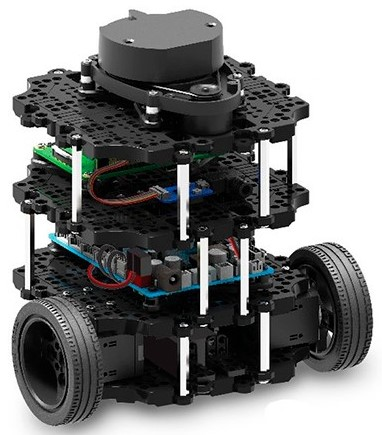
\includegraphics[width=\textwidth]{images/turtlebot3-burger.jpg}
    \end{minipage}%
    \begin{minipage}{.4\columnwidth}
        \centering
        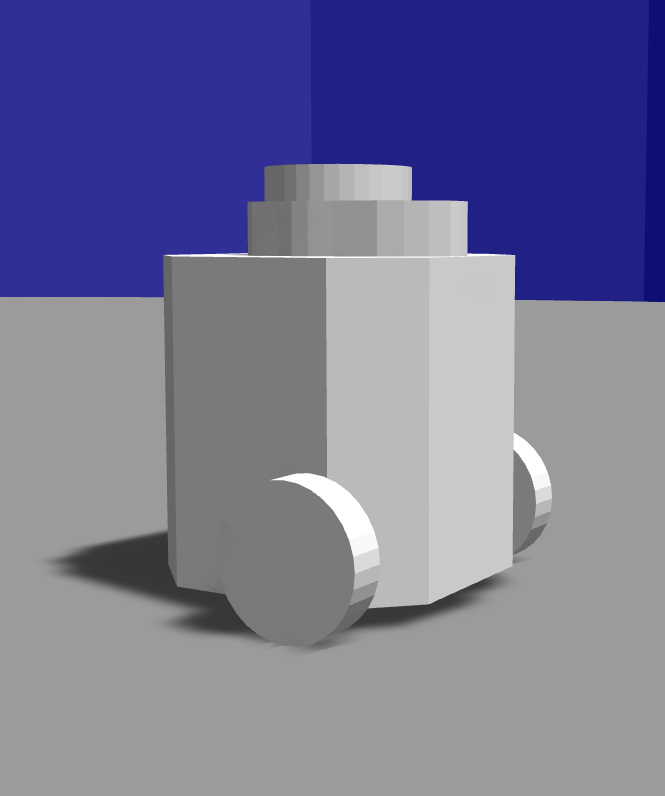
\includegraphics[width=\textwidth]{images/turtlebot3-burger-gazebo.png}
    \end{minipage}
    \caption{Turtlebot3 Burger in the real world (left) and in Gazebo (right)}
    \label{fig:robot-comparision}
\end{figure}

\subsection{The Environment}

The simulation environment is a question-marked shaped world. It was created using the Gazebo building
editor tool.

Project specifications specify that the bottom is straight with an edgy shape.

The figure \ref{fig:environment} is a visualization of the environment, in Gazebo:

\begin{figure}[h]
    \centering
    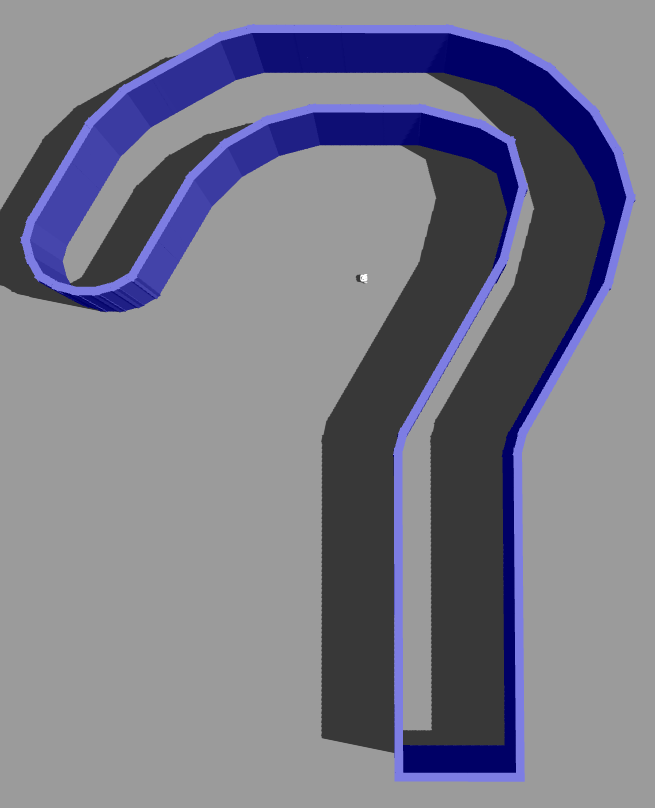
\includegraphics[width=0.3\textwidth]{images/world.png}
    \caption{The simulation world}
    \label{fig:environment}
\end{figure}

\subsection{Packages}

Inside our workspace, two packages were created: \emph{my\textunderscore reactive\textunderscore robot} and \emph{my\textunderscore controller}.

The first package:
\begin{itemize}
    \item Launches Gazebo, by running both \emph{gzserver.launch.py} and \emph{gzclient.launch.py}
    \item Publishes the robot state with the \emph{robot\textunderscore state\textunderscore publisher} node
    \item Spawns our Turtlebot3 robot in the simulation environment, with the \emph{spawn\textunderscore entity.py} service,
          from the package \emph{gazebo\textunderscore ros}
\end{itemize}

The second package, as the name suggests, is responsible for controlling the robot. It contains the following nodes:
\begin{itemize}
    \item \emph{scan\textunderscore to\textunderscore velocity\textunderscore node}: This node subscribes to
          the \emph{scan} topic, which contains the LIDAR data, and publishes the velocity commands to
          the \emph{cmd\textunderscore vel} topic, which controls the robot's wheels.
    \item \emph{spin \textunderscore randomly \textunderscore node}: This node is a workaround that we created to allow for a random initial
          robot orientation. It spins the robot randomly for a few seconds and then stops it.
\end{itemize}

The robot's initial position and pose are random but are constrained to the round area of the question mark.

\subsection{How to Run the Simulation}\label{sec:run}

To run the simulation, you will need the following ROS packages/dependencies:

\begin{itemize}
    \item \emph{turtlebot3\textunderscore gazebo}: This package contains the Turtlebot3 models and the Gazebo plugins.
    \item \emph{gazebo\textunderscore ros}: This package contains the Gazebo ROS interface.
\end{itemize}

Assure that you have the necessary dependencies and that you have sourced your ROS distribution's setup file. Please refer to the README file in the \href{https://github.com/carlosverissimo3001/FEUP-RI-PROJ/}{project's repository}, if you're having any issues with this process.

\vskip 0.1in

\textbf{Build the package and source the setup file}:

\begin{enumerate}
    \item \texttt{cd FEUP-RI-PROJ} - Go to the project's root directory
    \item \texttt{colcon build --symlink-install} - Build the packages
    \item \texttt{source install/setup.bash} - Source the setup file
    \item \texttt{export TURTLEBOT3\textunderscore MODEL=burger} - Set the Turtlebot3 model.
          You can change this to \emph{waffle} or \emph{waffle\textunderscore pi.}
\end{enumerate}

\vskip 0.1in

\textbf{Run the simulation}:

\begin{enumerate}
    \item Open two terminal windows.
    \item Run \texttt{ros2 launch my\textunderscore reactive\textunderscore robot launch.py} in one of them.
\end{enumerate}

This will launch Gazebo and spawn the robot in the simulation environment. Please wait for Gazebo to load before running the next command.

In the other terminal window, run \texttt{ros2 run my\textunderscore controller controller\textunderscore node}.
This will launch the nodes that control the robot.

\vskip 0.1in

Please note that we set up Gazebo so that it starts with a paused state. This means that the simulation will not start
until you press the play button in Gazebo's GUI.

\subsection{Implementation}

In addition to the tangible physical limitations of the robot, the robot controller must adhere to a primary constraint: it must operate without any recollection of past actions and/or states. Keeping this constraint in focus, the controller script is structured into three primary conditional evaluations:
\begin{enumerate}
    \item The controller checks if the robot has reached the final position.  
    \item Is the robot lost.
    \item The robot confirms it is within follow distance from the closest wall.
    \begin{enumerate}
        \item If it is too far away, then the robot will turn and face the wall, moving closer to it.
        \item If it is close enough, then it will enter the follow wall algorithm.
    \end{enumerate}
\end{enumerate}

\subsubsection{Final Position}

The robot has reached the final position when it is directly at the center bottom of the question mark.

In order for the robot to recognize that it reached the center of the wall both of the first and last LIDARs that detect a wall need to detect the wall at the same distance.

Additionally, for the robot to recognize that the wall it has reached is the bottom wall of the question mark, the calculated length of the detected wall has to match the length of the actual bottom wall. In order to achieve this, we decided to use the law of sines, this law was chosen because of the data we had: a) we have the distance from the robot to the two edges of the wall; b) we have the angle between the robot and both edges of the wall and c) we had the guarantee that the other two angles of the triangle were equal because the distance to both edges of the wall is the same.

\begin{figure}[h]
    \centering
    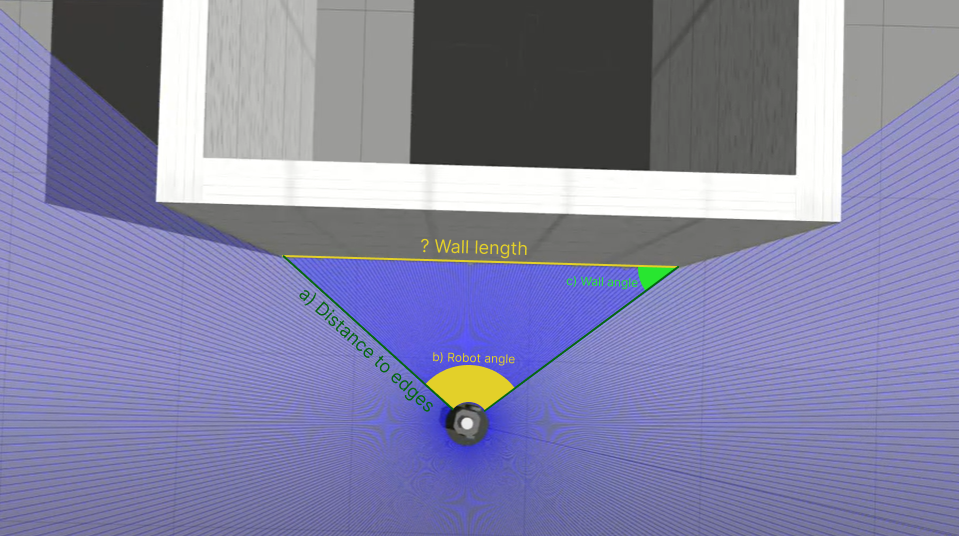
\includegraphics[width=.47\textwidth]          {images/robotEndCalc.png}
    \label{fig:robot-end-calculation}
    \caption{Data needed to compute robot's end position}
\end{figure}

\subsubsection{Lost Robot}
The robot is considered lost when no walls are detected in its LIDAR scans.

In this scenario, given that the robot lacks a concrete sense of direction, our approach was to maintain continuous forward movement. This particular state doesn't carry significant contextual significance, and it is not anticipated to happen during a standard program iteration.

\subsubsection{Move to Wall}
In order to better follow a wall the robot should move closer to it before entering the follow wall algorithm.

To enhance the robot's ability to approach the wall, it's imperative that the robot aligns itself perpendicular to the specific wall it intends to move closer to. To achieve this, the robot should rotate so that any of its front LIDARs detect the wall in the closest proximity.

Once the robot is properly oriented towards the wall, it can proceed by moving directly forward.

To ensure the robot effectively reduces the distance between itself and the wall, we employ a spinning action in the direction that will require the least amount of rotation while, simultaneously, we apply a modest amount of forward movement in order to accelerate the overall process.

\subsubsection{Follow the Wall}
For the robot to follow the wall, it needs two conditions met, 1) it needs to be close to the actual wall, and 2) its left or right sensor needs to be perpendicular to the wall it wants to follow.

Given the simplicity of visually identifying the shortest trajectory, we have opted to designate the left sensors as the primary sensors for analysis.

In theory, for a robot to effectively track a trajectory parallel to a wall, it is essential that its left-front sensors consistently maintain the same distance from the wall as the corresponding left-back sensors.

Our follow-wall algorithm is divided into four main conditions:
\begin{enumerate}
    \item The left sensor is not detecting any wall. In this situation, the robot will spin in the direction that requires the least amount of rotation in order so that the left sensor detects a wall.
    \item The left sensor detects a wall to close to the robot. We prioritize the robot's safety by instructing it to execute a rightward spin while maintaining a slow forward pace to prevent collisions.
    \item The left-front sensor and the left-back sensor return the same distance to the wall. This is our main goal and the state we want to maintain the robot in, when this occurs the robot is travelling parallel to the wall and will move forward.
    \item The left-front sensor and the left-back sensor return different distances from the wall. In this situation, the robot should continue its forward motion while applying a slight spin to rectify this distance gap.
\end{enumerate}

\section{Experiments}

As previously stated, the robot's initial pose is random: the robot spawns randomly inside a circle area
with 1 meter of radius at X = 2 and Y = 2.5.

To randomize the robot's orientation, specifically its yaw, we created a workaround node that spins the robot
with a random angular velocity (z axis) for a few seconds and then stops it.
This node is called \emph{spin\textunderscore randomly\textunderscore node}.

We have ran two different experiments:
\begin{itemize}
    \item In the first one, the robot's position is fixed at X=2 and Y=2.5, and its orientation is variable.
    \item In a second experiment, it's orientation is fixed, and we randomize the spawn coordinates
\end{itemize}

\subsection{Experiment 1}

In order to test how the robot's starting orientation affects the loop-time, we have ran the simulation 10 times, only changing the yaw (orientation at z) values, that range from -1 to 1, with a step of 0.2.

The table below shows the loop time in regards to the yaw value.


Another way to visualize this data is in an radar chart, with this chart the user can better understand in what orientation the robot performed worse and what the change  between each orientation is. 

\subsection{Experiment 2}

The second experiment tests the robot's performance, at different initial spawn positions.

\begin{figure}[h]
    \centering
    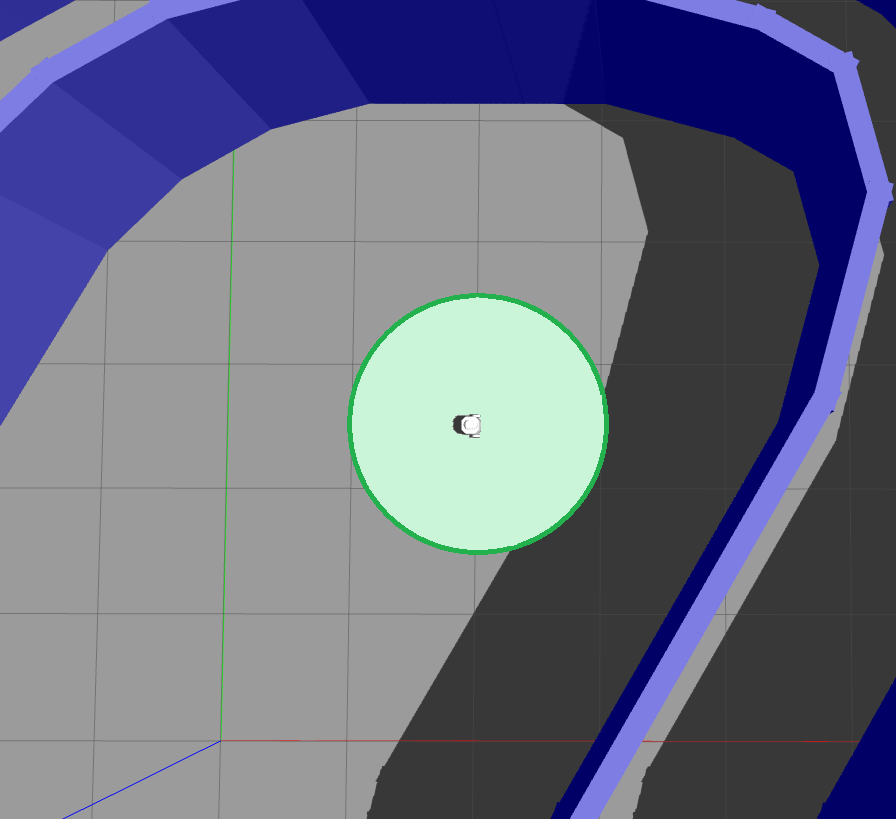
\includegraphics[width=0.3\textwidth]{images/spawn-positions.png}
    \caption{The robot's initial position}
    \label{fig:initial-position}
\end{figure}

The green area in figure \ref{fig:initial-position} shows the possible initial position of the robot.
We've conducted this experiment 10 times, and the robot's orientation was fixed at 0.0 (facing right on the image).


\section{Results and Discussion}

\subsection{Experiment 1}

The goal of this experiment was to analyse how much of an effect the orientation of the robot relatively to the closest wall affects it's travel time.

As previously mentioned, the robot's position was fixed at X=2.0 and Y=2.5. When viewed from a bird's-eye perspective, the closest walls to this point are situated either to the right or at the top. Consequently, it was anticipated that the robot would require more time when facing the bottom-left direction, as evidenced by the maximum time taken when the robot's yawn rotation was set to 0.6.

This result aligns with our expectations, based on the design of our robot's controller. However, it may not immediately appear intuitive to a first-time observer. When examining the robot's trajectory, the orientation often ends up being close to 0.6 while it follows the initial curved wall inside the question mark. This behavior arises from the specific distance we agreed our robot needs to maintain from the wall in order to follow it effectively. If we were to increase this threshold, along with expanding the LIDAR's detection range, it is expected that the value of 0.6 should shift from being the slowest to the fastest time, as the robot wouldn't need to make significant adjustments to its initial rotation, unlike other orientations.

\subsection{Experiment 2}

The goal of this experiment was to analyse how much of an effect the initial position of the robot relatively to the closest wall affects it's overall travel time.

As observable in table \ref{table: exp2}, the worst runs are the 6th and 7th runs, to no surprise, as these runs are the ones where the robot spawns in a way that puts the top wall as the closest wall to the robot.

The fastest runs, on the other hand, are the 4th and 9th runs, where the robot spawns in a way that puts the right/bottom walls as the closest walls to the robot.

The behavior is more clearly depicted through the heat map shown in Figure \ref{fig:position_heat_map}.

\section{Conclusions and Future Work}

To sum up, this project has proven to be a great way to practice using the Robot Operating System (ROS) and the Gazebo simulation environment. It offered insights into autonomous navigation, sensor-actuator integration, and real-time robotic behavior, making it a useful chance to dig into the complexities of ROS robotics.

Nevertheless, it's important to recognize that more time than expected was spent correctly setting up and launching the project. This demonstrates how crucial it is to comprehend the nuances of ROS and Gazebo in order to execute projects without any problems. 

\subsection{Future Work}
Future work might include improving the robot's ability to spawn inside the environment's walls, which would add a new element of difficulty to the navigation challenge. Consider a situation in which the robot must find its way from within the labyrinthine structure to the bottom of the '?' form, opening up new avenues for study and development.

Moreover, there are a few improvements that our robot would welcome, namely:
\begin{enumerate}
    \item Presently, the robot adheres to a fixed rotation value. To improve efficiency, it could be advantageous to adjust the rotation based on the specific situation it encounters. For instance, when the robot needs to perform a 180-degree spin, a higher rotation value could expedite this process.
    \item Similarly, the robot's movement speed could be made adaptive. It should vary depending on the circumstances. However, it's essential to establish an upper limit to prevent potential collisions.
    \item The robot's current approach to stopping when it reaches the middle of the bottom wall lacks a specific endpoint. To enhance its path-following capabilities, it might be valuable to designate a predetermined endpoint for the robot to navigate towards. 
\end{enumerate}

\section{Acknowledgments}

First and foremost, we would like to express our gratitude for the collaboration and cooperation we have maintained throughout this relatively brief yet intricate task.

Secondly, we thank the course's professors, for their guidance and support throughout the development
of this project.

Finally, We would also like to extend our gratitude to the authors of the ROS packages that we used in this project.

%\begin{thebibliography}{00}
    %\bibitem{b1} G. Eason, B. Noble, and I. N. Sneddon, ``On certain integrals of Lipschitz-Hankel type involving products of Bessel functions,'' Phil. Trans. Roy. Soc. London, vol. A247, pp. 529--551, April 1955.
    %\bibitem{b2} J. Clerk Maxwell, A Treatise on Electricity and Magnetism, 3rd ed., vol. 2. Oxford: Clarendon, 1892, pp.68--73.
    %\bibitem{b3} I. S. Jacobs and C. P. Bean, ``Fine particles, thin films and exchange anisotropy,'' in Magnetism, vol. III, G. T. Rado and H. Suhl, Eds. New York: Academic, 1963, pp. 271--350.
    %\bibitem{b4} K. Elissa, ``Title of paper if known,'' unpublished.
    %\bibitem{b5} R. Nicole, ``Title of paper with only first word capitalized,'' J. Name Stand. Abbrev., in press.
    %\bibitem{b6} Y. Yorozu, M. Hirano, K. Oka, and Y. Tagawa, ``Electron spectroscopy studies on magneto-optical media and plastic substrate interface,'' IEEE Transl. J. Magn. Japan, vol. 2, pp. 740--741, August 1987 [Digests 9th Annual Conf. Magnetics Japan, p. 301, 1982].
    %\bibitem{b7} M. Young, The Technical Writer's Handbook. Mill Valley, CA: University Science, 1989.
%\end{thebibliography}

\appendices

\section{Tables} \label{tables}

\begin{table}[H]
    \caption{Experiment 1 : Results}
    \label{table: exp1}
    \begin{tabularx}{\columnwidth}{@{} *{2}{C} @{}}
        \toprule
        Yaw (Z-Orientation) & Time to Finish (s) \\
        \midrule
        -1.0 & 95              \\
        -0.8 & 90              \\
        -0.6 & 92              \\
        -0.4 & 91              \\
        -0.2 & 91              \\
         0.0 & 93              \\
         0.2 & 87              \\
         0.4 & 91              \\
         0.6 & 103             \\
         0.8 & 94              \\
        \bottomrule
    \end{tabularx}
\end{table}

\begin{table}[H]
    \caption{Experiment 2 : Results}
    \label{table: exp2}
    \begin{tabularx}{\columnwidth}{@{} *{3}{C} @{}}
        \toprule
        X & Y & Time to Finish (s) \\
        \midrule
        1.81 & 2.44 & 94           \\
        1.92 & 2.34 & 90           \\
        2.43 & 2.88 & 94           \\
        1.87 & 2.39 & 94           \\
        2.52 & 2.39 & 82           \\
        2.21 & 2.90 & 91           \\
        1.59 & 3.19 & 130          \\
        1.99 & 3.49 & 126          \\
        2.46 & 1.67 & 83           \\
        1.62 & 2.67 & 102          \\
        \bottomrule
    \end{tabularx}
\end{table}

\newpage

\section{Images}
\label{images}

\begin{figure}[H]
    \centering
    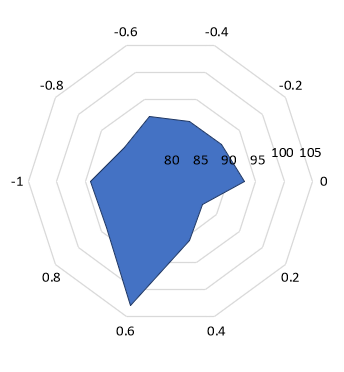
\includegraphics[width=0.4\textwidth]{images/Rotation_timings.png}
    \caption{How the initial rotation affects time taken in seconds}
    \label{fig:rotation_radar_chart}
\end{figure}

%% CHANGE TO HEATMAP
\begin{figure}[H]
    \centering
    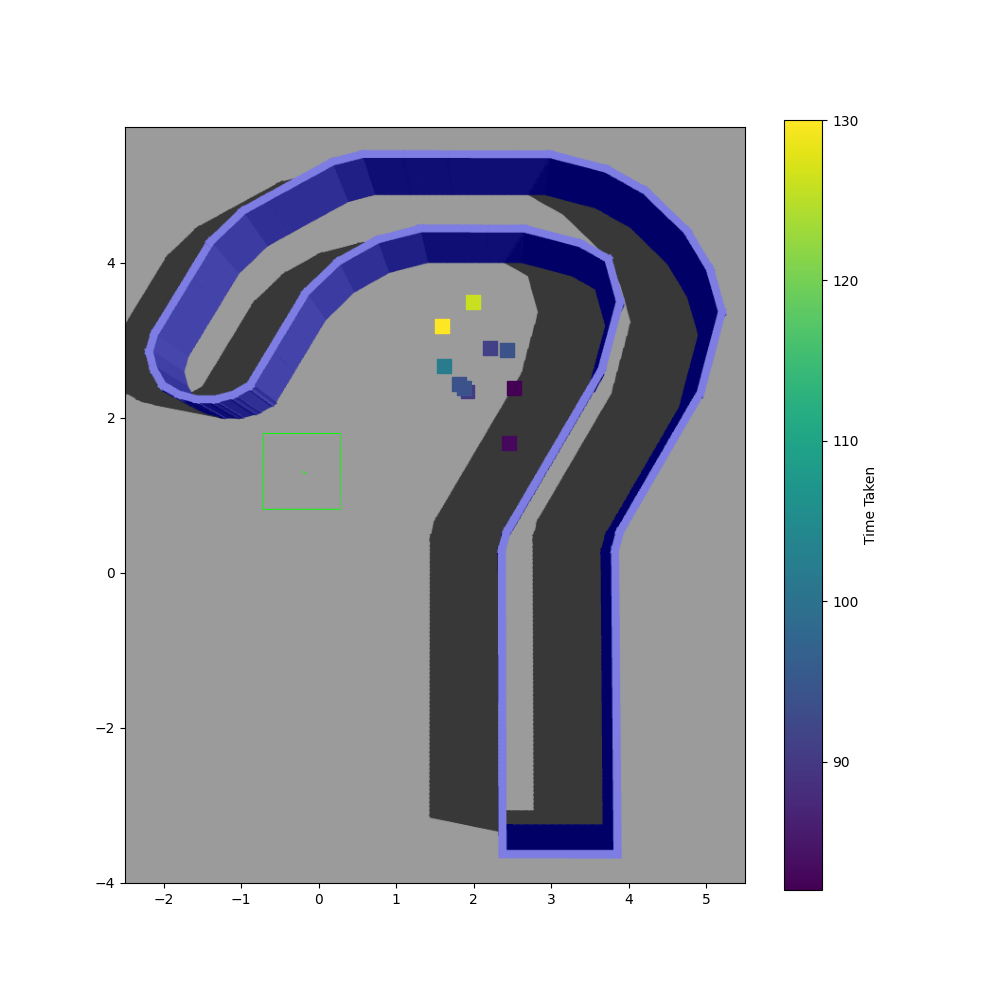
\includegraphics[width=0.45\textwidth]{images/heatMap_position.png}
    \caption{How the initial position affects time taken in seconds}
    \label{fig:position_heat_map}
\end{figure}

\end{document}
